\documentclass[exam, 12pt]{wvwcdocs}

\course{}
\examnum{The Final Exam You've Been Waiting For}
\examdate{July 3, 2026}
\usepackage[T1]{fontenc}
\usepackage{tkz-berge}
\definecolor{codegreen}{rgb}{0,0.6,0}
\definecolor{codegray}{rgb}{0.5,0.5,0.5}
\definecolor{codepurple}{rgb}{0.58,0,0.82}
\definecolor{backcolour}{rgb}{0.95,0.95,0.92}

\lstdefinestyle{mystyle}{
    backgroundcolor=\color{backcolour},
    commentstyle=\color{codegreen},
    keywordstyle=\color{magenta},
    numberstyle=\tiny\color{codegray},
    stringstyle=\color{codepurple},
    basicstyle=\footnotesize,
    breakatwhitespace=false,
    breaklines=true,
    captionpos=b,
    keepspaces=true,
    numbers=left,
    numbersep=5pt,
    showspaces=false,
    showstringspaces=false,
    showtabs=false,
    tabsize=2
}

\lstset{style=mystyle}

\begin{document}
\lstset{language=python}
% These commands specify the coverpage
\begin{coverpages}

    \noindent
    This test contains \numpages\ pages (not including this cover page) and \numquestions\ problems.
    The point value of each problem is indicated in the margin.
    Please check to see if any pages are missing.

    \noindent
    The following rules apply:

    \begin{minipage}[t]{.5\linewidth}
        \vspace{0pt}
        \begin{itemize}
            % \item \textbf{This test is closed book}.
            % You may not use a textbook, notes or other resources including (but not limited to) electronic/smart devices during this test.
            % Usage of any of these during the test \textbf{will be considered grounds for an academic integrity violation} and will be dealt with accordingly.

            \item \textbf{Any code must be Python compatible}.
                  In particular, if you're writing code to represent a mathematical expression then you must write valid Python code as opposed to valid mathematical notation.
                  As an example, you should write \texttt{pi} instead of $\pi$ if you need to use the constant $\pi$ in your code.

            \item \textbf{Organize your work} in a reasonably neat and coherent way in the space provided.
                  Work scattered all over the page without a clear ordering will receive very little credit.

                  % \item \textbf{You must show relevant work}.
                  % A correct answer, unsupported by calculations, explanation or algebraic work may not receive credit; an incorrect answer supported by substantially correct calculations and explanations might still receive significant partial credit.

            \item \textbf{You do not need to simplify your answers} unless otherwise stated.
        \end{itemize}

        \vspace{1cm}

        Indicate that you have read and understood these rules by printing your name below.

        \vspace{1cm}

        \makebox[\textwidth]{\textsc{Name(s)}:\enspace\hrulefill}
    \end{minipage}
    \hspace{.5cm}
    \begin{minipage}[t]{.4\linewidth}
        \vspace{0pt}
        % \cellwidth{1pt}
        \vqword{Problem}
        % \gradetable[v][pages]
        \combinedgradetable[v][pages]  % Use [pages] to have grading table by page instead of question. Bonus points option
        % \partialgradetable{range1}[v][pages]  % Use [pages] to have grading table by page instead of question

    \end{minipage}

    \newpage % End of cover page
    $\,$
\end{coverpages}

\begin{questions}
    \question[10]\label{ques:check-group}
    Consider all possible three letter ``words'' that can be made from the letters \( \set{A, B, C} \).
    Consider the following two actions:
    \begin{enumerate}
    \item You can swap the first and last letters of the word.
    \item You can remove the second letter.
          \end{enumerate}
          Explain why these actions do \textit{not} form a group.


          \question[10]\label{ques:symmetry-group-non-square-rectangle}
          Complete the following.
          \begin{parts}
              \qpart\label{part:symmetry-group-actions}
              List the actions in the symmetry group of a non-square rectangle.
              You can describe these actions geometrically (i.e., using rotations/flips) or algebraically (i.e., using permutations).


              \qpart\label{part:mattress-group}
              Suppose you have a non-square and rectangular mattress that needs to be flipped occasionally.
              You would like to find a single flip or rotation that you could use repeatedly to cycle through all four of the different positions of the mattress.
              Is this possible?


          \end{parts}

          \question[10]\label{ques:group-with-eight-elements}
          Describe how you could construct a group with exactly five actions.
          \textit{Hint}: use a geometric object!


          \question[10]\label{ques:symmetry-group}
          List all of the actions in the symmetry group of the symbol ``I''.


          \question[10]\label{ques:permutations}  Let
          \[
              \sigma = \left(
              \begin{array}{llllll}
                  1 & 2 & 3 & 4 & \\
                  3 & 1 & 4 & 2 &
              \end{array}
              \right), \rho = \left(
              \begin{array}{llllll}
                  1 & 2 & 3 & 4 \\
                  3 & 4 & 2 & 1
              \end{array}
              \right)
          \]
          \begin{parts}
              \qpart\label{part:cycle-notation}
              Write down what \( \sigma \) and \( \rho \) are using cycle notation.


              \qpart\label{part:evaluating-composition}
              Find \( \sigma\rho \).


              \qpart\label{part:parity-permutation}
              Is \( \sigma \) an even permutation?


          \end{parts}

          \question[10]\label{ques:hamiltonian-group}
          The \textbf{Hamiltonian group} (also called the \textbf{quaternion group}) is a group with elements \[ \set{1, -1, i, -i, j, -j, k, -k} \] and Cayley table (i.e., multiplication table!
          ) given by
          \begin{center}
              \begin{tblr}{%
                      cells={r},
                      row{odd} = {bg=azure9},
                      row{1} = {bg=azure3, fg=white, font=\sffamily},
                      column{1} = {bg=azure3, fg=white, font=\sffamily},
                      rows = {mode=math},
                  }
                  \mathbb{H} & 1  & -1 & i  & -i & j  & -j & k  & -k \\
                  1          & 1  & -1 & i  & -i & j  & -j & k  & -k \\
                  -1         & -1 & 1  & -i & i  & -j & j  & -k & k  \\
                  i          & i  & -i & -1 & 1  & k  & -k & -j & j  \\
                  -i         & -i & i  & 1  & -1 & -k & k  & j  & -j \\
                  j          & j  & -j & -k & k  & -1 & 1  & i  & -i \\
                  -j         & -j & j  & k  & -k & 1  & -1 & -i & i  \\
                  k          & k  & -k & j  & -j & -i & i  & -1 & 1  \\
                  -k         & -k & k  & -j & j  & i  & -i & 1  & -1 \\
              \end{tblr}
          \end{center}
          Answer the following questions.
          \begin{parts}
              \qpart\label{part:i-squared}
              Explain how to use the above table to show that \( i^2 = -1 \) in this group.


              \qpart\label{part:ij-product}
              Is \( ij \) equal to \( ji \) in this group?


          \end{parts}

          \question[10]\label{ques:friendship-graph}
          A friendship graph is a graph where any pair of vertices have exactly one neighbor (i.e., ``friend'') in common.
          \begin{parts}
              \qpart\label{part:examples-friendship}
              Draw two different examples of friendship graphs.


              \qpart\label{part:friendship-party}
              Suppose you are at a party where any two people know exactly one other person at the party.
              Explain why there must be someone at the party who knows everybody else.


          \end{parts}

          \question[10]\label{ques:name-graph}
          Draw a graph where the vertices are the elements of the Hamiltonian group (see question~\ref{ques:hamiltonian-group}) and the edges correspond to pairs of elements that multiply to \( 1 \) or \( -1 \).


          \question[10]\label{ques:tournaments}
          Suppose that seven teams are playing in a tournament.
          Is it possible for each team to play exactly five of the other teams?


          \question[10]\label{ques:huffman-code}  Consider the following Huffman code:
          \begin{center}
              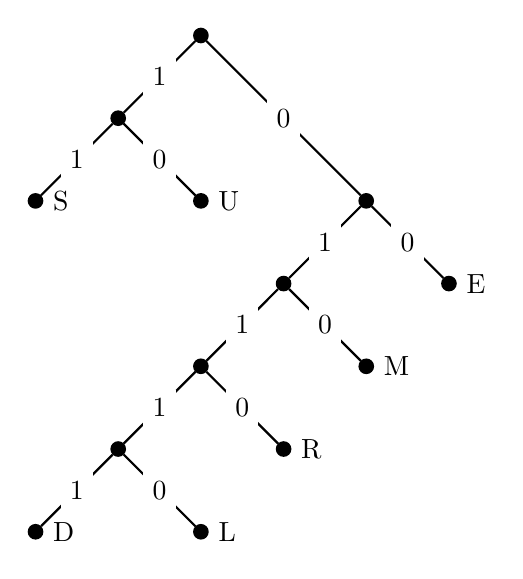
\begin{tikzpicture}[scale=.35]
                  \GraphInit[vstyle=Classic]
                  \tikzset{VertexStyle/.style = {shape = circle,fill = black,minimum size = 2pt,inner sep=2pt}}
                  % \SetVertexNormal
                  \SetGraphUnit{3}
                  \SetVertexNoLabel
                  \Vertex{O}
                  \SOWE(O){O1}
                  \Vertex[x = 6, y = -6]{O0}
                  \SOWE(O0){O01}
                  \SOWE(O01){O011}
                  \SOWE(O011){O0111}
                  \SetVertexLabel
                  \SOWE(O1){S}
                  \SOEA(O1){U}
                  \SOEA(O0){E}
                  \SOEA(O01){M}
                  \SOEA(O011){R}
                  \SOEA(O0111){L}
                  \SOWE(O0111){D}
                  \Edges[label={$1$}](O,O1,S)
                  \Edges[label={$1$}](O0,O01,O011,O0111,D)
                  \Edges[label={$0$}](O,O0,E)
                  \Edges[label={$0$}](O1,U)
                  \Edges[label={$0$}](O01,M)
                  \Edges[label={$0$}](O011,R)
                  \Edges[label={$0$}](O0111,L)
              \end{tikzpicture}
          \end{center}
          \begin{parts}
              \qpart\label{part:frequency}
              This Huffman code is based on some string of letters.
              What letter(s) do you think appeared the most in this string?
              What letter(s) do you think appeared the least?


              \qpart\label{part:summer}
              Decode the following string using the above code: \( 1110010010000110 \).


          \end{parts}

          \question[10]\label{ques:sympy-permutations}
          Let \( \sigma = (12458) \).
          \begin{parts}
              \qpart\label{part:sympy-code}
              Complete the following block with code that will implement the above permutation in Python.
              \begin{lstlisting}[gobble=22]
                      # Complete the line of code below.
                      from sympy.combinatorics import

                      # Complete the line of code below.
                      sigma =

                  \end{lstlisting}


              \qpart\label{part:product}
              Find the product of \( \sigma \) with itself ten times in a row.
              You are \textit{highly encouraged} to use Python for this!


          \end{parts}

          \question[10]\label{ques:group-in-python}
          Suppose we want to form a group from the cycles \( \sigma = (12458) \) and \( \rho = (179) \).
          \begin{parts}
              \qpart\label{part:sympy-code}
              How would you create this group in SymPy?


              \qpart\label{part:number-of-elements}
              How many elements are in the group you just created?

          \end{parts}

          \question[10]\label{ques:rubik-cube-move-order}
          Suppose you take a Rubik's cube and you perform the following sequence of twists: \( F*L*U*R \).
          How many times would you have to perform this sequence of moves before you get back to where you started?
          You are \textit{highly} encouraged to make use of the provided \texttt{rubiks-cube-group.py} file!


          \question[10]\label{ques:graph-adjacency-matrix} Using the adjacency matrix from the provided file \texttt{adjacency\textunderscore{}matrix.py}, answer the following questions:
          \begin{parts}
              \qpart\label{part:code-for-graph}
              What Python code would you need to add to the file to have it create *and show* the graph corresponding to the adjacency matrix \( A \)?


              \qpart\label{part:graph-drawing}
              Draw the graph that corresponds to the adjacency matrix \( A \).


              \qpart\label{part:walks}
              How many walks are there from vertex \( 0 \) to vertex \( 3 \) of length five?


          \end{parts}

          \bonusquestion[5] What is (probably) my first name?



\end{questions}
\end{document}

%%% Local Variables:
%%% mode: LaTeX
%%% TeX-master: t
%%% End:
